\chapter{经典信息、可逆动力学与矩阵}

\lectureoverview{量子力学要求我们在超出日常直觉训练范围的领域中进行推理。因此，我们提前一步，从经典信息开始：比特、位形以及可逆更新定律。同样的讨论自然引向矢量与矩阵，它们将为量子比特提供语言。}

\section{为错误世界建立的直觉}

我们的物理直觉由来已久。早在任何人写下方程之前，追逐猎物的动物就必须估计相对速度和方向。如果一头狮子正在逼近一只羚羊，狮子是在对不断变化的间距作出反应，因此是以一种隐含的方式对相对速度作出反应。能够很好地处理这类判断的神经系统受到了青睐；处理得差的那些没有留下多少后代。我们关于运动的所谓常识，大多是在这个平凡世界中训练出来的。

这份遗产很有用，但很狭窄。日常生活中没有任何东西以接近光速运动，因此进化没有提供关于相对论时空的本能。物理学家先学习抽象几何，之后才获得对它的新直觉。量子力学还要更难。我们熟悉的粒子图景来自石头和箭：在每一瞬间物体都有一个位置，位置的相继形成一条轨迹，位置的变化定义速度。电子并不迁就我们去符合那幅图景。位置不确定性和经典轨迹的缺失，在塑造我们感官的经验中没有对应物。

这种直觉的失败并不存在悖论。只有当适应石头、动物和中等速度的本能不知何故预先了解电子时，才会存在悖论。正确的回应是从一小组精确规则出发建立一种不同的直觉。这里的重点不会是通常经由波动力学和Schr\"odinger方程的路线。我们将集中关注量子力学的逻辑结构和量子信息。在追问量子比特是什么之前，我们必须确切理解普通比特做什么。

\section{比特与信息量}

物理学与信息密不可分。有时这种信息由一个实数表示，但最简单的一则信息是对一个只有两种可能答案的问题的回答：是或否，正面或反面，上或下。

\begin{definition}
一个\emph{经典比特}是一个恰好有两种可能答案的物理问题。
\end{definition}

我们可以把这些答案标记为\(0\)和\(1\)。这些标记本身不带有内在含义；任何两个不同的符号都可以。由于狄拉克记号很快就会变得不可或缺，即使它目前还是多余的，我们也先引入它：
\begin{equation}
  \ket{0},
  \qquad
  \ket{1}.
\end{equation}
竖线和尖括号构成一个\emph{ket}，即bra--ket的右半部分。仅仅因为我们改变了记号，并没有任何量子内容进入。

对于若干个可区分的比特，按固定顺序写出答案。例如，六枚可区分的硬币可以具有位形
\begin{equation}
  \ket{0\,1\,1\,0\,1\,0}.
\end{equation}
一旦顺序被理解，逗号就是可选的。一个比特有两种可能状态，两个比特有四种，每增加一个比特，数目就翻倍。因此，一个\(n\)比特系统有
\begin{equation}
  N_s=2^n
  \label{eq:l01-state-count}
\end{equation}
种状态。反过来，
\begin{equation}
  n=\log_2 N_s.
  \label{eq:l01-bits-from-states}
\end{equation}

式~\eqref{eq:l01-bits-from-states}提示了一个即使状态数不是二的幂也有用的定义：
\begin{equation}
  I=\log_2 N_s.
  \label{eq:l01-information}
\end{equation}
因此，一个六面骰子携带\(\log_2 6\)比特的信息。答案不必是整数。由二进制开关字面组装而成的系统将是方便的示例，但对数是更一般的度量。

\section{编码一个看似连续的世界}

比特并不局限于硬币。任何已知到有限精度的被测量量都可以写成一个有限二进制串。例如，假设一个房间的温度只要求达到选定的有效数字位数。把测得的值用二进制表示，并保留达到该精度所需的数字。更高的精度需要更长的串，但原理不变。

空间变化的场可以类似处理。把房间分成精细有序的格胞，以有限精度记录每个格胞中的场值，并把得到的二进制串连接起来。把格胞做得更小可以提高空间分辨率；保留更多二进制数字可以提高场值分辨率。温度场、电场和磁场都可以按这种方式编码到任何规定的有限精度。

粒子构型给出了一幅更加字面化的二进制图景。把空间细分为足够小的格子，使每个格子至多容纳一个粒子。赋值
\begin{equation}
  n_i=
  \begin{cases}
    1,&\text{cell \(i\) is occupied},\\
    0,&\text{cell \(i\) is empty}.
  \end{cases}
  \label{eq:l01-occupancy-bit}
\end{equation}
完整的构型就是有序串
\begin{equation}
  \ket{n_1n_2n_3\cdots}.
\end{equation}
这是对一连串是或否问题的极长回答：第一个格子里有粒子吗，第二个格子里有吗，如此等等？这是游戏\emph{二十问}的物理版本，只不过问题的数目可能极其巨大。

这一构造解释了为什么数字计算机能够模拟物理。计算机存储的是有限字符串，而有限分辨率则把被测量的量和场恰好变成这样的字符串。通过细化格点、时间步长或保留的位数，可以系统地改进这一近似。

\begin{classroomqa}
\lecturetimestamp{00:29:43}
\audiencequestion{温度表示的精度是任意的吗？}
\lecturerresponse{它是根据我们想要的近似来选取的。有限字符串给出有限精度；保留更多二进制位则给出更精细的近似。这里并没有声称有限字符串能精确指定任意的经典实数。}
\end{classroomqa}

\begin{classroomqa}
\lecturetimestamp{00:30:11}
\audiencequestion{对于一般的实数，尤其是无理数，情况如何？}
\lecturerresponse{一个精确的实数可能需要无穷多位。有些有理数的二进制展开是循环的，而一般的无理数展开则永不终止。真实的计算机总是只保留有限多位数字。要点在于，任何指定的有限精度都可以被编码，而不是说每一个经典实数都有有限的精确描述。}
\end{classroomqa}

\section{状态与运动定律}

到目前为止，我们描述的是系统在某一瞬间的情况。运动还需要第二个要素。

\begin{definition}
\emph{构型}是系统在指定瞬间的完整状态。离散时间运动定律是一条把每个构型映射到其后一个时间步的构型的规则。
\end{definition}

这一区分是初等的，但至关重要。电子分布的一幅快照是一个构型；它还不是一条轨道。如果把空间换成格点、把时间换成序列\(t_0,t_1,t_2,\ldots\)，那么运动就是如下相继关系
\begin{equation}
  \ket{s(t_0)}
  \longmapsto
  \ket{s(t_1)}
  \longmapsto
  \ket{s(t_2)}
  \longmapsto\cdots.
  \label{eq:l01-discrete-motion}
\end{equation}
因此，一个物理模型既需要一组可能的状态，也需要一条更新规则。

\begin{classroomqa}
\lecturetimestamp{00:31:12}
\audiencequestion{这种格子描述如何说明电子在轨道上运动？}
\lecturerresponse{首先只指定某一瞬间的构型：哪些格子被占据，如果模型包含原子核，则原子核固定不动。然后把时间离散化。轨道运动就是把一个占据串更新为下一个占据串的规则。由于格子的排序，这条规则可能很复杂，但它仍然是对信息的更新。}
\end{classroomqa}

画出一个抽象的\emph{状态空间}会有所帮助。这个空间中的每个点都表示一个完整的构型，而不是普通空间中的一个位置。一个\(10\times10\)占据格点包含一百个比特，因而有\(2^{100}\)种可能的构型。\editorialnote{口头讲授在展开这个例子时曾简略地说成\(10^{100}\)；比特数确定了其本意应为\(2^{100}\)。}这些构型中的每一个都是状态空间中的一个单独的点。

对于一个比特，只有两个点。恒等定律使两者都保持不变：
\begin{equation}
  0\mapsto0,
  \qquad
  1\mapsto1.
  \label{eq:l01-identity-update}
\end{equation}
另一种可逆的可能性是把它们互换：
\begin{equation}
  0\mapsto1,
  \qquad
  1\mapsto0.
  \label{eq:l01-flip-update}
\end{equation}
这就是一个翻转-翻转。一个自由演化的物理实例并不像手动操作的灯开关那样直接，因为干预会扩大系统。昼夜提供了一个近似的两态循环；单摆也在两个极端之间交替，尽管它的完整状态还包括所有中间位置和速度。

\begin{classroomqa}
\lecturetimestamp{00:40:38}
\audiencequestion{普通的灯开关会是翻转-翻转定律的一个例子吗？}
\lecturerresponse{如果是由人来拨动它，那就不是，因为此时开关并不是自行演化的；人属于被扩大了的动力学系统。我们要寻找的是一个封闭系统，其自身的定律使它的状态交替变化。昼夜提示了这一想法，而单摆则提醒我们，真实的例子通常不止两个状态。}
\end{classroomqa}

一个两比特系统有四种构型。一条更新定律可以把全部四种构型沿一个循环带走。另一条更新定律则可以由两个各自独立的二循环组成。这些是构型逻辑空间中的回路，而不一定是物理空间中的回路。箭头指定了定律：无论系统从哪里开始，沿着箭头走就告诉我们它此后的历史。

\section{可逆性与区分的保持}

并非每个箭头图都具有相同的物理地位。考虑一条规则，其中两个不同的状态合并为同一个后继：
\begin{equation}
  a\mapsto c,
  \qquad
  b\mapsto c.
  \label{eq:l01-merging-update}
\end{equation}
无论我们从\(a\)还是\(b\)出发，下一个状态都是确定的，但到达\(c\)之后，我们无法确定发生的是哪一个过去。\(a\)与\(b\)之间的区别已经消失。

\begin{figure}[htbp]
\centering
\includegraphics[width=0.82\linewidth]{lecture_01_figure_02.png}
\caption{在关于可逆性的讨论中，黑板上保留着几个更新图。闭合循环与合并模式并存，量子术语\emph{幺正性}写在它们旁边。}
\lectureframe{00:53:21}
\end{figure}

\begin{figure}[htbp]
\centering
\begin{tikzpicture}[>=Latex,thick,node distance=1.15cm]
  \node[circle,fill,inner sep=1.8pt,label=above:\(1\)] (r1) {};
  \node[circle,fill,inner sep=1.8pt,right=of r1,label=above:\(2\)] (r2) {};
  \node[circle,fill,inner sep=1.8pt,below=of r2,label=below:\(3\)] (r3) {};
  \node[circle,fill,inner sep=1.8pt,left=of r3,label=below:\(4\)] (r4) {};
  \draw[->] (r1) -- (r2);
  \draw[->] (r2) -- (r3);
  \draw[->] (r3) -- (r4);
  \draw[->] (r4) -- (r1);
  \node[below=0.5cm of r4,anchor=north west] {\small reversible cycle};

  \node[circle,fill,inner sep=1.8pt,right=4.2cm of r1,label=above:\(a\)] (a) {};
  \node[circle,fill,inner sep=1.8pt,below=1.25cm of a,label=below:\(b\)] (b) {};
  \node[circle,fill,inner sep=1.8pt,right=1.6cm of a,yshift=-0.625cm,label=above:\(c\)] (c) {};
  \node[circle,fill,inner sep=1.8pt,right=of c,label=above:\(d\)] (d) {};
  \draw[->] (a) -- (c);
  \draw[->] (b) -- (c);
  \draw[->] (c) -- (d);
  \node[below=0.55cm of b,anchor=north west] {\small information-losing merge};
\end{tikzpicture}
\caption{可逆规则为每个状态指定一个前驱和一个后继。合并规则具有唯一的未来，但过去是模糊的。}
\end{figure}

当所有自由度都被保留时，基本经典动力学不允许这种损失。所需性质包含两半：
\begin{equation}
  \boxed{\begin{gathered}
    \text{one unique future and one unique past}\\
    \text{for every state}
  \end{gathered}.}
  \label{eq:l01-reversibility}
\end{equation}
对于有限状态空间，更新因此必须是一个置换。每个状态恰好有一条出射箭头和恰好一条入射箭头，因此该图分解为互不相交的循环。

\begin{classroomqa}
\lecturetimestamp{00:46:32}
\audiencequestion{合并图有什么不同？}
\lecturerresponse{它并非完全由循环组成。更根本地说，在合并状态发现系统并不能告诉我们它先前是哪个前驱。我们可以构造未来，但无法重建过去。一个比特的历史区别已经丢失。}
\end{classroomqa}

这个概念是\emph{时间可逆性}，而不一定是精确的时间反演对称性。顺时针循环具有确定的前进方向。原始定律不会使系统逆时针运动，但存在一个逆定律会使其如此。精确的时间反演对称性提出了一个额外问题：在施加适当的反演操作之后，是否得到相同的动力学定律？仅就可逆性而言，它只问历史能否被唯一地反向运行。

\begin{classroomqa}
\lecturetimestamp{00:49:58}
\audiencequestion{过去的唯一性就是时间反演对称性吗？}
\lecturerresponse{不完全是。循环的箭头可能只指向一个方向，因此定律具有方向性。可逆性意味着通过反转每个箭头可以构造出一个定义良好的逆定律。它本身并不说明逆定律与原始定律相同。}
\end{classroomqa}

我们也不应通过在合并状态处放置两条出射箭头来修复一个不可逆图。那会以另一种方式使反向运动变得模糊：系统将需要一个概率性指令，也许在\(30\%\)的时间选择一条分支，在\(70\%\)的时间选择另一条。我们仍然在构造确定性经典动力学，其中一个当前状态决定一个未来和一个过去。

每个真实系统归根结底都是量子力学的。为什么大物体看起来是经典的，以及为什么它们的量子替代方案变得难以观测，是以后的问题。相应的量子原理将保留相同的逻辑核心。半开玩笑地说，人们可以把过去与未来的唯一性称为\emph{唯一性}。它的实际名称是\emph{幺正性}：量子演化可以唯一地向前或向后运行。

\section{表观信息丢失与粗粒化}

宏观经验似乎与可逆性相矛盾。把密封房间中所有气体分子放在左角，然后释放它们。不久气体就充满房间。如果改为从右角开始，最终的宏观图像看起来相同。这两个不同的初始状态合并了吗？

只有在我们丢弃细节之后才会如此。微观状态指定了每个分子。如果能够以足够的精度跟踪每个位置和速度，那么反转这些运动将区分这两种制备。在实践中，计算极其困难，而且所需精度迅速增长，但实践上的无能为力并不是根本性的抹除。宏观陈述\emph{空气充满房间}把数量巨大的不同微观构型识别为一个粗粒化状态。

热力学第二定律正是在这里进入。我们失去区分详细状态的能力，是因为我们没有跟踪所有微观变量。信息看似消失，是因为我们的描述是粗粒化的，而不是因为细粒度的确定性定律合并了不同的点。

\begin{classroomqa}
\lecturetimestamp{00:56:11}
\audiencequestion{追踪经典房间中所有分子是否需要无穷多个比特？}
\lecturerresponse{若要求精确的经典描述，答案是肯定的。位置和速度是实数，而对一个混沌的多粒子系统追踪更长时间就需要越来越高的精度。量子力学改变了这一结论：对于一个能量有界的封闭区域，物理上可区分的描述可以是离散的，而不是任意一串精确的经典实数。}
\end{classroomqa}

这个问题并非只是学术性的。黑洞能否摧毁信息曾争论了数十年；斯蒂芬·霍金最初主张它可以。那场争论所问的是：这种表面上的合并是否只是另一种粗粒化描述，还是对量子幺正性的真正违反。在量子力学提供精确语言之前，我们不会解决它，但它揭示了有多少东西依赖于那些简单的箭头图。

\section{行、列与内积}

在用量子比特取代经典比特之前，我们需要少量线性代数。就目前的目的而言，向量可以简单地视为一个有限的有序实数列表。一个四分量向量可以水平地写成
\begin{equation}
  A^{\mathsf T}=(A_1,A_2,A_3,A_4),
  \label{eq:l01-row-vector}
\end{equation}
或者垂直地写成
\begin{equation}
  A=
  \begin{pmatrix}
    A_1\\ A_2\\ A_3\\ A_4
  \end{pmatrix}.
  \label{eq:l01-column-vector}
\end{equation}
\emph{四维}一词仅仅意味着有四个分量。无需在普通空间中想象一个箭头。水平对象是行向量，垂直对象是列向量。

\begin{figure}[htbp]
\centering
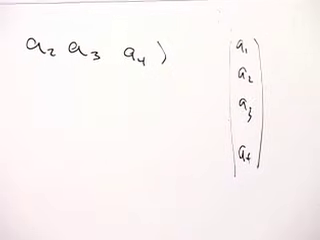
\includegraphics[width=0.92\linewidth]{lecture_01_figure_03.png}
\caption{同样的分量被写成一行和一列。在这个阶段它们是实数，因此不涉及复共轭。}
\lectureframe{01:03:05}
\end{figure}

\begin{classroomqa}
\lecturetimestamp{01:03:14}
\audiencequestion{行向量不就是列向量的匕首吗？}
\lecturerresponse{一旦分量是复数，那将是正确的语言。那时转置必须伴随复共轭。目前元素是实数，所以我们只需区分行的排列与列的排列。}
\end{classroomqa}

设
\begin{equation}
  B=(B_1,B_2,B_3,B_4)
\end{equation}
为一个行，其元素个数与列\(A\)相同。它们的乘积通过匹配位置并求和来定义：
\begin{align}
  BA
  &=
  (B_1,B_2,B_3,B_4)
  \begin{pmatrix}
    A_1\\ A_2\\ A_3\\ A_4
  \end{pmatrix}\\
  &=B_1A_1+B_2A_2+B_3A_3+B_4A_4.
  \label{eq:l01-inner-product}
\end{align}
结果是一个数，而不是另一个向量或矩阵。在抽象向量空间中，这个运算称为内积。

\begin{classroomqa}
\lecturetimestamp{01:06:44}
\audiencequestion{这是点积吗？}
\lecturerresponse{是的。对于三维空间中的普通向量，它就是熟悉的点积。\emph{内积}这个名称强调，同样的行乘列运算适用于任何有限维的向量空间。}
\end{classroomqa}

\section{矩阵作为更新状态的机器}

矩阵是一个方形数字阵列，它作用于一个向量以产生另一个向量。把它想象成一台机器：输入旧的列，应用一条固定规则，得到一个新的列。在四维中，
\begin{equation}
  M=
  \begin{pmatrix}
    M_{11}&M_{12}&M_{13}&M_{14}\\
    M_{21}&M_{22}&M_{23}&M_{24}\\
    M_{31}&M_{32}&M_{33}&M_{34}\\
    M_{41}&M_{42}&M_{43}&M_{44}
  \end{pmatrix}.
  \label{eq:l01-general-matrix}
\end{equation}
第一个指标标记行，第二个指标标记列。可以把\(M\)视为列的集合，也可以视为行的集合；这两种观点都将有用。

要计算\(A'=MA\)，取\(M\)的每一行与输入列的内积：
\begin{equation}
  A'_i=(MA)_i=\sum_{j=1}^{4}M_{ij}A_j.
  \label{eq:l01-matrix-vector}
\end{equation}
例如，
\begin{align}
  A'_1&=M_{11}A_1+M_{12}A_2+M_{13}A_3+M_{14}A_4,\\
  A'_2&=M_{21}A_1+M_{22}A_2+M_{23}A_3+M_{24}A_4.
\end{align}
第三和第四个元素按同样的模式得出。

\begin{figure}[htbp]
\centering
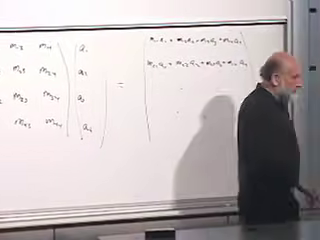
\includegraphics[width=0.94\linewidth]{lecture_01_figure_04.png}
\caption{矩阵逐行作用于列向量。前两个输出分量在黑板上被明确展开。}
\lectureframe{01:12:45}
\end{figure}

\subsection{编码一个经典位形}

假设一个系统有四种可能的状态。用独热列来表示它们
\begin{equation}
  e_1=
  \begin{pmatrix}1\\0\\0\\0\end{pmatrix},
  \quad
  e_2=
  \begin{pmatrix}0\\1\\0\\0\end{pmatrix},
  \quad
  e_3=
  \begin{pmatrix}0\\0\\1\\0\end{pmatrix},
  \quad
  e_4=
  \begin{pmatrix}0\\0\\0\\1\end{pmatrix}.
  \label{eq:l01-one-hot}
\end{equation}
单个\(1\)的位置告诉我们当前存在的是哪一种经典位形。

考虑循环更新
\begin{equation}
  1\longrightarrow2\longrightarrow3\longrightarrow4\longrightarrow1.
  \label{eq:l01-four-cycle}
\end{equation}
它由下式表示
\begin{equation}
  P=
  \begin{pmatrix}
    0&0&0&1\\
    1&0&0&0\\
    0&1&0&0\\
    0&0&1&0
  \end{pmatrix}.
  \label{eq:l01-permutation-matrix}
\end{equation}
确实，
\begin{equation}
  \begin{aligned}
    Pe_1&=e_2, & Pe_2&=e_3,\\
    Pe_3&=e_4, & Pe_4&=e_1.
  \end{aligned}
\end{equation}
黑板上的构造在书写过程中被修正，先是五个状态，然后是四个状态。方程~\eqref{eq:l01-permutation-matrix}记录的是最终确定的循环规则，而不是被放弃的中间阵列。

同一个矩阵作用于任意列：
\begin{equation}
  P
  \begin{pmatrix}A\\B\\C\\D\end{pmatrix}
  =
  \begin{pmatrix}D\\A\\B\\C\end{pmatrix}.
  \label{eq:l01-cyclic-shift}
\end{equation}
对于经典状态，只有一个分量为\(1\)，但允许一般元素则揭示了底层的线性运算。经典确定性更新使用特殊的零一矩阵，每一行和每一列中都有一个\(1\)。量子力学将保留矩阵演化，同时极大地扩大允许的元素。

\subsection{复合就是矩阵乘法}

如果一个时间步是
\begin{equation}
  V'=MV,
\end{equation}
那么第二次应用给出
\begin{equation}
  V''=MV'=M(MV)=M^2V.
  \label{eq:l01-two-updates}
\end{equation}
因此，矩阵相乘并非任意的代数消遣。它复合的是物理更新。五个时间步由\(M^5\)表示。

对于两个 \(2\times2\) 矩阵
\begin{equation}
  M=
  \begin{pmatrix}
    M_{11}&M_{12}\\
    M_{21}&M_{22}
  \end{pmatrix},
  \qquad
  N=
  \begin{pmatrix}
    N_{11}&N_{12}\\
    N_{21}&N_{22}
  \end{pmatrix},
\end{equation}
乘积 \(C=MN\) 的元素为
\begin{equation}
  C_{ij}=\sum_k M_{ik}N_{kj}.
  \label{eq:l01-matrix-product}
\end{equation}
特别地，
\begin{align}
  C_{11}&=M_{11}N_{11}+M_{12}N_{21},\\
  C_{12}&=M_{11}N_{12}+M_{12}N_{22},\\
  C_{21}&=M_{21}N_{11}+M_{22}N_{21},\\
  C_{22}&=M_{21}N_{12}+M_{22}N_{22}.
\end{align}
每个元素都是左矩阵的一行乘以右矩阵的一列。等价地，用 \(M\) 作用于 \(N\) 的每一列，并将所得各列并排放置。

\begin{figure}[htbp]
\centering
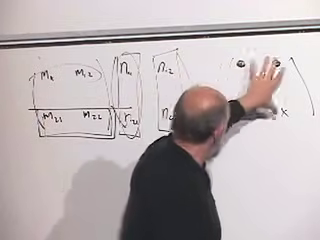
\includegraphics[width=0.86\linewidth]{lecture_01_figure_05.png}
\caption{矩阵乘法被组织为重复的矩阵--列乘法。第一行与第二个矩阵的各列被标出，以显示乘积的每个元素来自何处。}
\lectureframe{01:26:30}
\end{figure}

行向量也可以从左侧作用。若 \(B=(B_1,\ldots,B_4)\)，则 \(BM\) 是另一个行向量，且
\begin{equation}
  (BM)_j=\sum_i B_iM_{ij}.
  \label{eq:l01-row-times-matrix}
\end{equation}
规则同样是行乘以列。形状记录了结果：
\begin{equation}
\begin{array}{c@{\qquad}c}
\text{row}\times\text{column}&=\text{number},\\
\text{matrix}\times\text{column}&=\text{column},\\
\text{row}\times\text{matrix}&=\text{row},\\
\text{matrix}\times\text{matrix}&=\text{matrix}.
\end{array}
\label{eq:l01-shape-rules}
\end{equation}

这些运算值得用小的数值 \(2\times2\) 和 \(3\times3\) 例子来练习。连同一点微积分，行--列乘法是前方量子力学所需的主要新数学习惯。

\begin{classroomqa}
\lecturetimestamp{01:31:50}
\audiencequestion{可逆性对更新矩阵施加了什么限制？}
\lecturerresponse{它必须具有逆。逆矩阵实现反向更新，并将每个状态带回其唯一的前驱。并非每个矩阵都可逆，因此这套代数再现了先前用箭头图作出的区分。对于循环例子，\(P^{-1}=P^3\) 且 \(P^4=\mathbb{1}\)。}
\end{classroomqa}

\section{为什么在量子比特之前先准备代数？}

第一个小时用比特和可逆箭头给出了确定性经典物理的定性描述。余下的数学把这一描述转化为一种能够经受向量子力学过渡的形式。一个构型变成一列；一步定律变成一个矩阵；重复的时间演化变成矩阵的乘积；可逆性变成逆的存在。

我们尚未使用任何量子规则。这种延迟是有意为之。接下来，我们将经典备选 \(\ket{0}\) 和 \(\ket{1}\) 替换为量子比特，并追问可能出现哪些新状态。这里引入的行向量、列向量、内积和矩阵，随后将揭示为什么量子信息与经典比特串如此截然不同。

\begin{classroomqa}
\lecturetimestamp{01:34:00}
\audiencequestion{为什么在说明其用途之前引入所有这些矩阵代数？}
\lecturerresponse{定性问题先出现：确定性物理应当如何由状态和更新定律来表示？这套代数是为下一步做准备。一旦引入量子比特，这些操作将不再显得脱离语境；它们将成为量子态及其演化的自然语言。}
\end{classroomqa}